\chap{ASR-A30-P75}

\begin{table}[ht!]
    \centering
    \begin{tabular}{| p{2.0cm} | p{1.6cm} | p{1.6cm} | p{1.6cm} | p{1.6cm} | p{1.6cm} | p{1.6cm} | p{1.6cm} | p{2.0cm} | }
    \hline

	Expansion [\%] & 0-0.0001mm & 0.0001-0.001mm & 0.001-0.01mm & 0.01-0.1mm & 0.1+mm & Sum \\ \hline

    0.0699 &	512896 &	310203 &	2118 &  	0 &	0 &	825217\\ \hline
    0.1936 &	579249 &	570671 &	62649 &	    0 &	0 &	1212569\\ \hline
    0.4223 &	603448 &	681853 &	173985 &	275 &	0 &	1459561\\ \hline
    0.8832 &	629798 &	771779 &	299364 &	8393 &	0 &	1709334\\ \hline
    1.3224 &	652189 &	833253 &	376456 &	29725 &	0 &	1891623\\ \hline

    \end{tabular}
    \caption{Number of Cracked Faces in Different Crack Width}
    \label{}
\end{table}

%% ASR_A30_P75_3 Internal Stress
\begin{figure}[ht!]
\centering
    %*******
    %*******
    \begin{subfigure}{.25\textwidth}
      \centering
      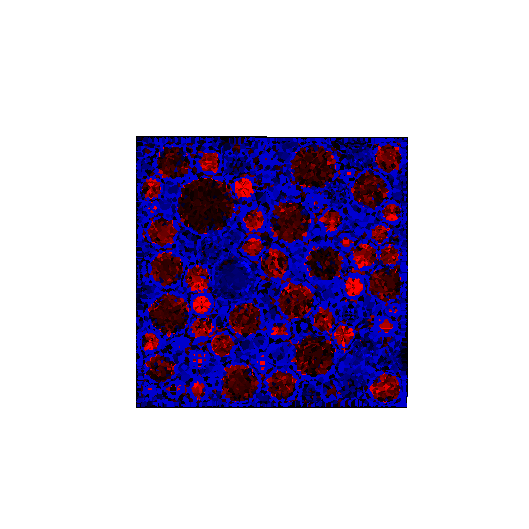
\includegraphics[width=1.0\linewidth]{Files/exp_3D/ASR/A30P75_1_s5.png}
      \caption{0.0699\% Expansion\\Internal Stress Step 5}
    \end{subfigure}%
    %*******
    \begin{subfigure}{.25\textwidth}
      \centering
      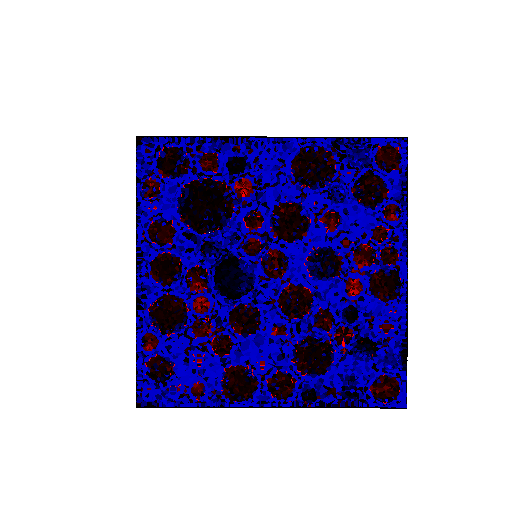
\includegraphics[width=1.0\linewidth]{Files/exp_3D/ASR/A30P75_1_s10.png}
      \caption{0.0699\% Expansion\\Internal Stress Step 10}
    \end{subfigure}%
    %*******
    \begin{subfigure}{.25\textwidth}
      \centering
      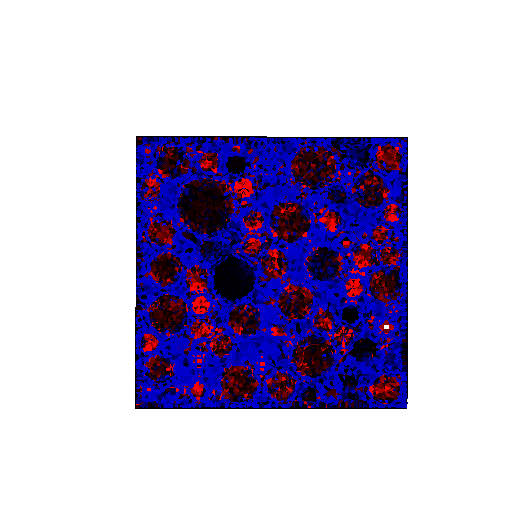
\includegraphics[width=1.0\linewidth]{Files/exp_3D/ASR/A30P75_1_s15.png}
      \caption{0.0699\% Expansion\\Internal Stress Step 15}
    \end{subfigure}%
    %*******
    \begin{subfigure}{.25\textwidth}
      \centering
      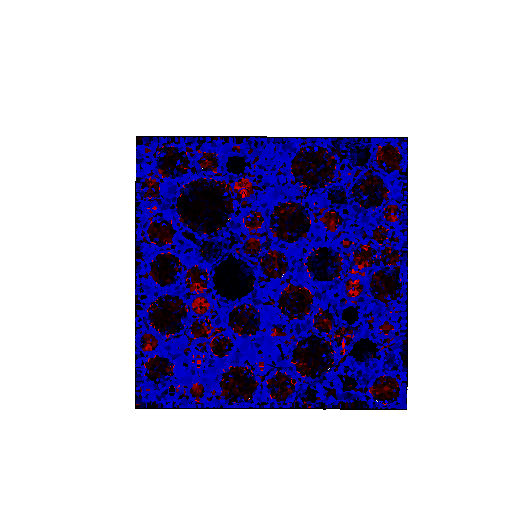
\includegraphics[width=1.0\linewidth]{Files/exp_3D/ASR/A30P75_1_stress.png}
      \caption{0.0699\% Expansion\\Internal Stress Step 20}
    \end{subfigure}
    %*******
    %*******
    \begin{subfigure}{.25\textwidth}
      \centering
      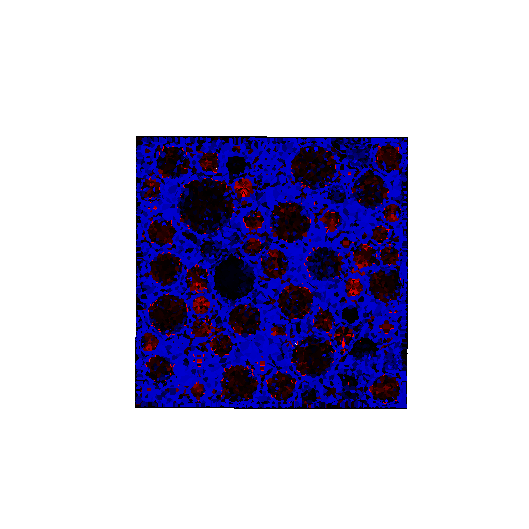
\includegraphics[width=1.0\linewidth]{Files/exp_3D/ASR/A30P75_2_s5.png}
      \caption{0.1936\% Expansion\\Internal Stress Step 5}
    \end{subfigure}%
    %*******
    \begin{subfigure}{.25\textwidth}
      \centering
      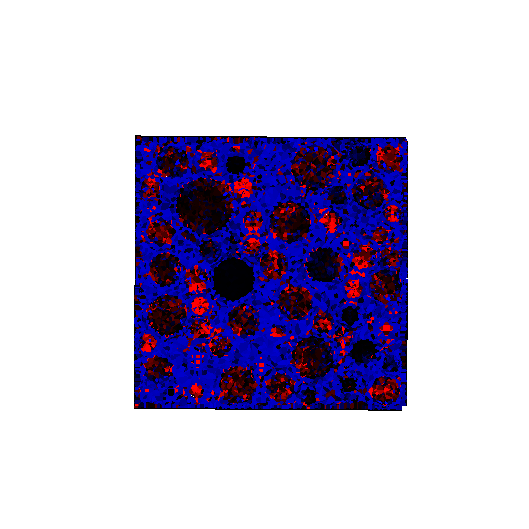
\includegraphics[width=1.0\linewidth]{Files/exp_3D/ASR/A30P75_2_s10.png}
      \caption{0.1936\% Expansion\\Internal Stress Step 10}
    \end{subfigure}%
    %*******
    \begin{subfigure}{.25\textwidth}
      \centering
      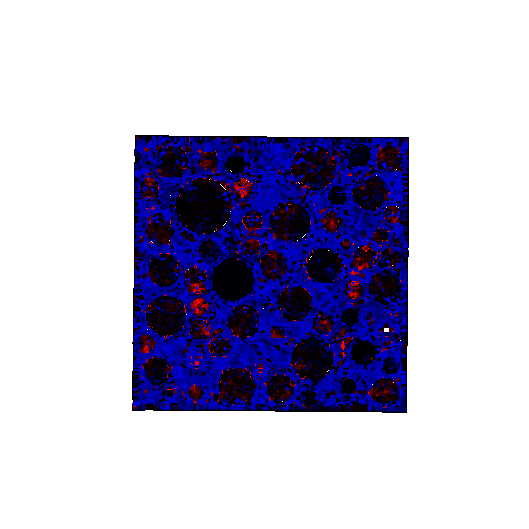
\includegraphics[width=1.0\linewidth]{Files/exp_3D/ASR/A30P75_2_s15.png}
      \caption{0.1936\% Expansion\\Internal Stress Step 15}
    \end{subfigure}%
    %*******
    \begin{subfigure}{.25\textwidth}
      \centering
      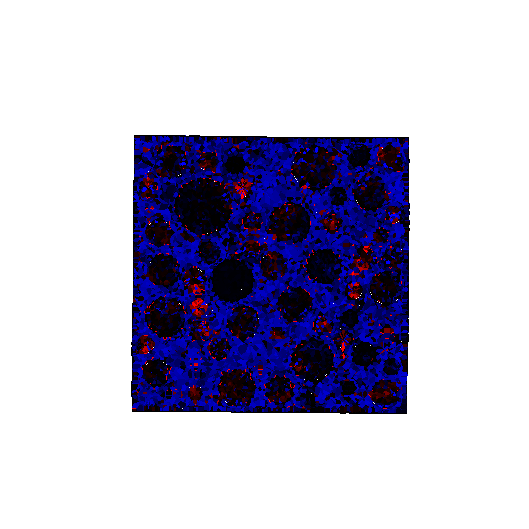
\includegraphics[width=1.0\linewidth]{Files/exp_3D/ASR/A30P75_2_stress.png}
      \caption{0.1936\% Expansion\\Internal Stress Step 20}
    \end{subfigure}
    %*******
    %*******
    \begin{subfigure}{.25\textwidth}
      \centering
      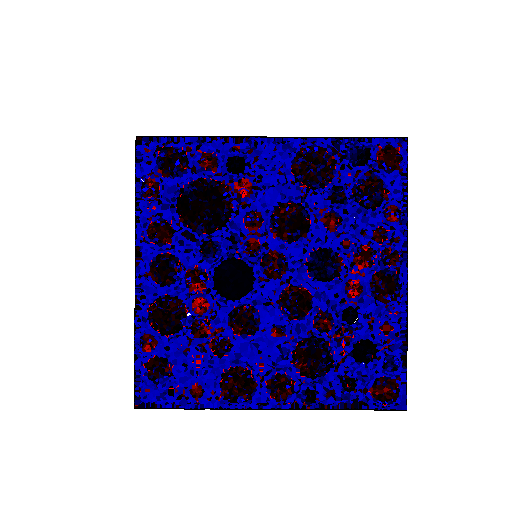
\includegraphics[width=1.0\linewidth]{Files/exp_3D/ASR/A30P75_3_s5.png}
      \caption{0.4223\% Expansion\\Internal Stress Step 5}
    \end{subfigure}%
    %*******
    \begin{subfigure}{.25\textwidth}
      \centering
      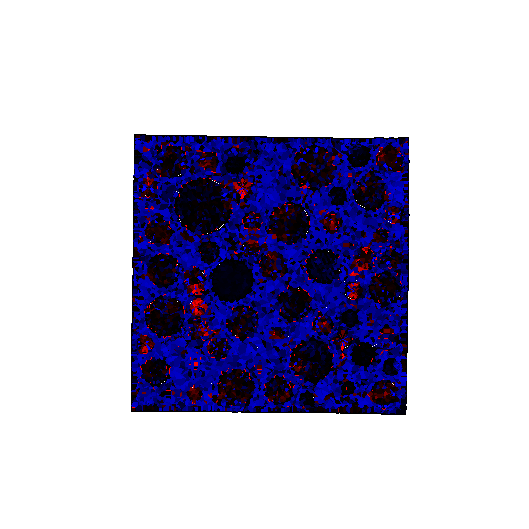
\includegraphics[width=1.0\linewidth]{Files/exp_3D/ASR/A30P75_3_s10.png}
      \caption{0.4223\% Expansion\\Internal Stress Step 10}
    \end{subfigure}%
    %*******
    \begin{subfigure}{.25\textwidth}
      \centering
      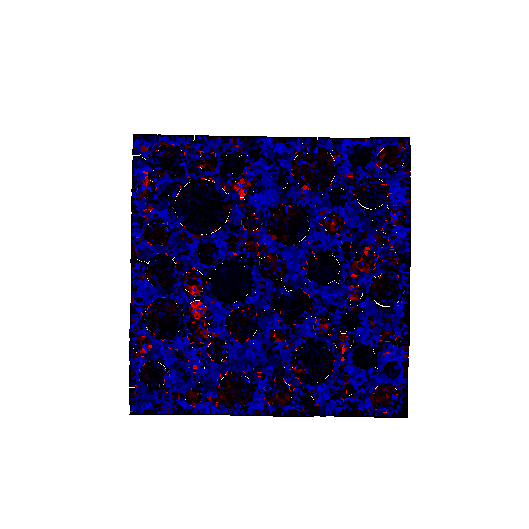
\includegraphics[width=1.0\linewidth]{Files/exp_3D/ASR/A30P75_3_s15.png}
      \caption{0.4223\% Expansion\\Internal Stress Step 15}
    \end{subfigure}%
    %*******
    \begin{subfigure}{.25\textwidth}
      \centering
      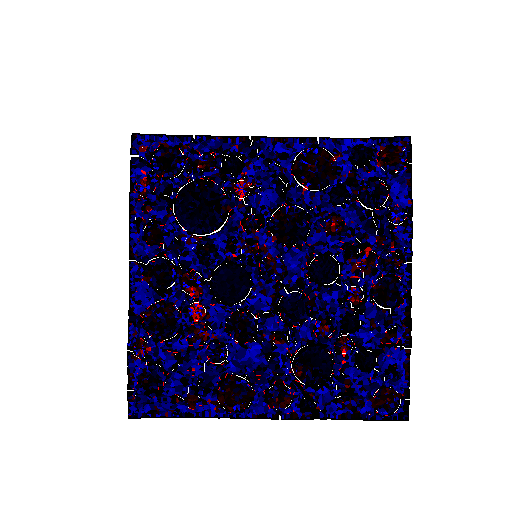
\includegraphics[width=1.0\linewidth]{Files/exp_3D/ASR/A30P75_3_stress.png}
      \caption{0.4223\% Expansion\\Internal Stress Step 20}
    \end{subfigure}
    %*******

    %*******
    \begin{subfigure}{.25\textwidth}
      \centering
      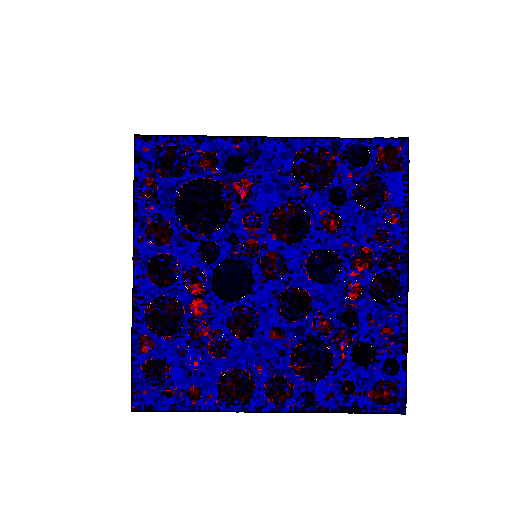
\includegraphics[width=1.0\linewidth]{Files/exp_3D/ASR/A30P75_4_s5.png}
      \caption{0.8832\% Expansion\\Internal Stress Step 5}
    \end{subfigure}%
    %*******
    \begin{subfigure}{.25\textwidth}
      \centering
      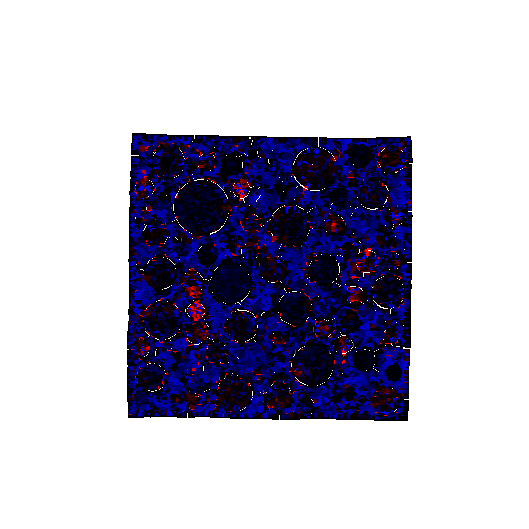
\includegraphics[width=1.0\linewidth]{Files/exp_3D/ASR/A30P75_4_s10.png}
      \caption{0.8832\% Expansion\\Internal Stress Step 10}
    \end{subfigure}%
    %*******
    \begin{subfigure}{.25\textwidth}
      \centering
      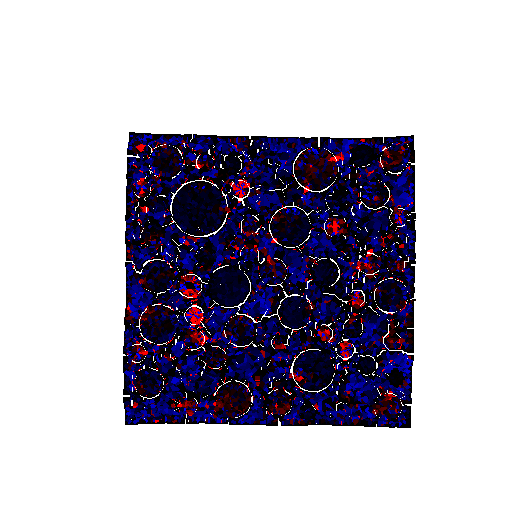
\includegraphics[width=1.0\linewidth]{Files/exp_3D/ASR/A30P75_4_s15.png}
      \caption{0.8832\% Expansion\\Internal Stress Step 15}
    \end{subfigure}%
    %*******
    \begin{subfigure}{.25\textwidth}
      \centering
      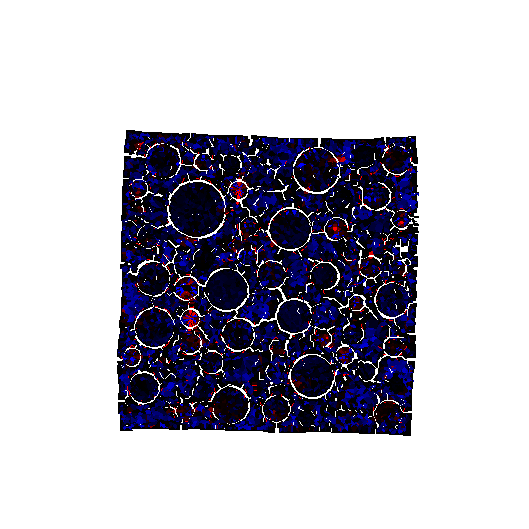
\includegraphics[width=1.0\linewidth]{Files/exp_3D/ASR/A30P75_4_stress.png}
      \caption{0.8832\% Expansion\\Internal Stress Step 20}
    \end{subfigure}
    %*******

    %*******
    \begin{subfigure}{.25\textwidth}
      \centering
      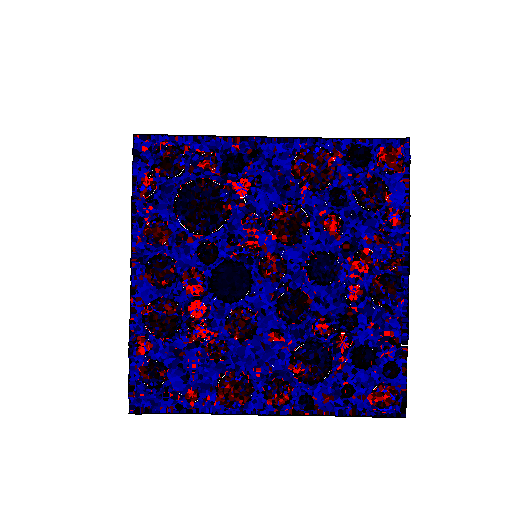
\includegraphics[width=1.0\linewidth]{Files/exp_3D/ASR/A30P75_5_s5.png}
      \caption{1.3224\% Expansion\\Internal Stress Step 5}
    \end{subfigure}%
    %*******
    \begin{subfigure}{.25\textwidth}
      \centering
      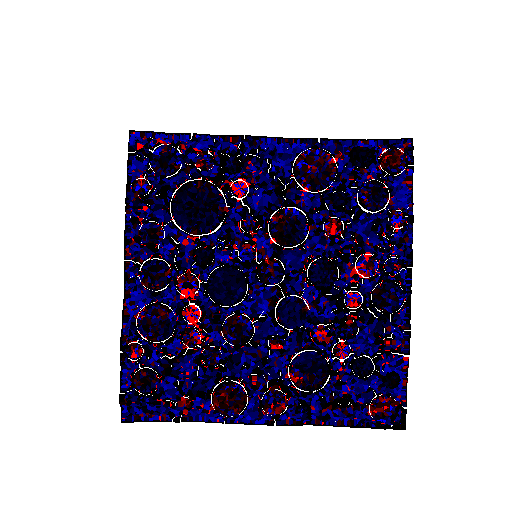
\includegraphics[width=1.0\linewidth]{Files/exp_3D/ASR/A30P75_5_s10.png}
      \caption{1.3224\% Expansion\\Internal Stress Step 10}
    \end{subfigure}%
    %*******
    \begin{subfigure}{.25\textwidth}
      \centering
      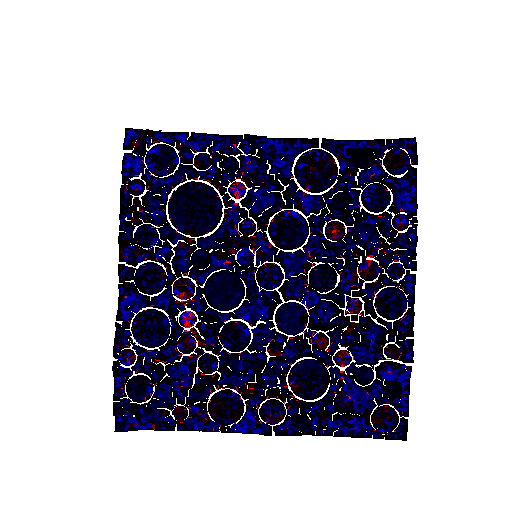
\includegraphics[width=1.0\linewidth]{Files/exp_3D/ASR/A30P75_5_s15.png}
      \caption{1.3224\% Expansion\\Internal Stress Step 15}
    \end{subfigure}%
    %*******
    \begin{subfigure}{.25\textwidth}
      \centering
      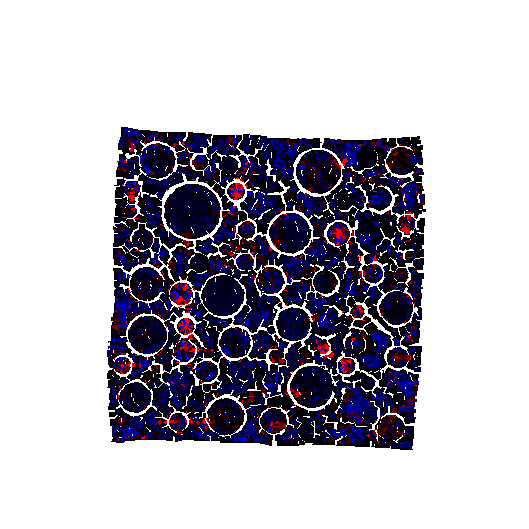
\includegraphics[width=1.0\linewidth]{Files/exp_3D/ASR/A30P75_5_stress.png}
      \caption{1.3224\% Expansion\\Internal Stress Step 20}
    \end{subfigure}
    %*******

\caption{Generation of Internal Stress for Expansion to Step 20(Final Expansion Step)}
\label{fig:A30_stress}
\end{figure}


\begin{figure}[ht!]
    \centering
    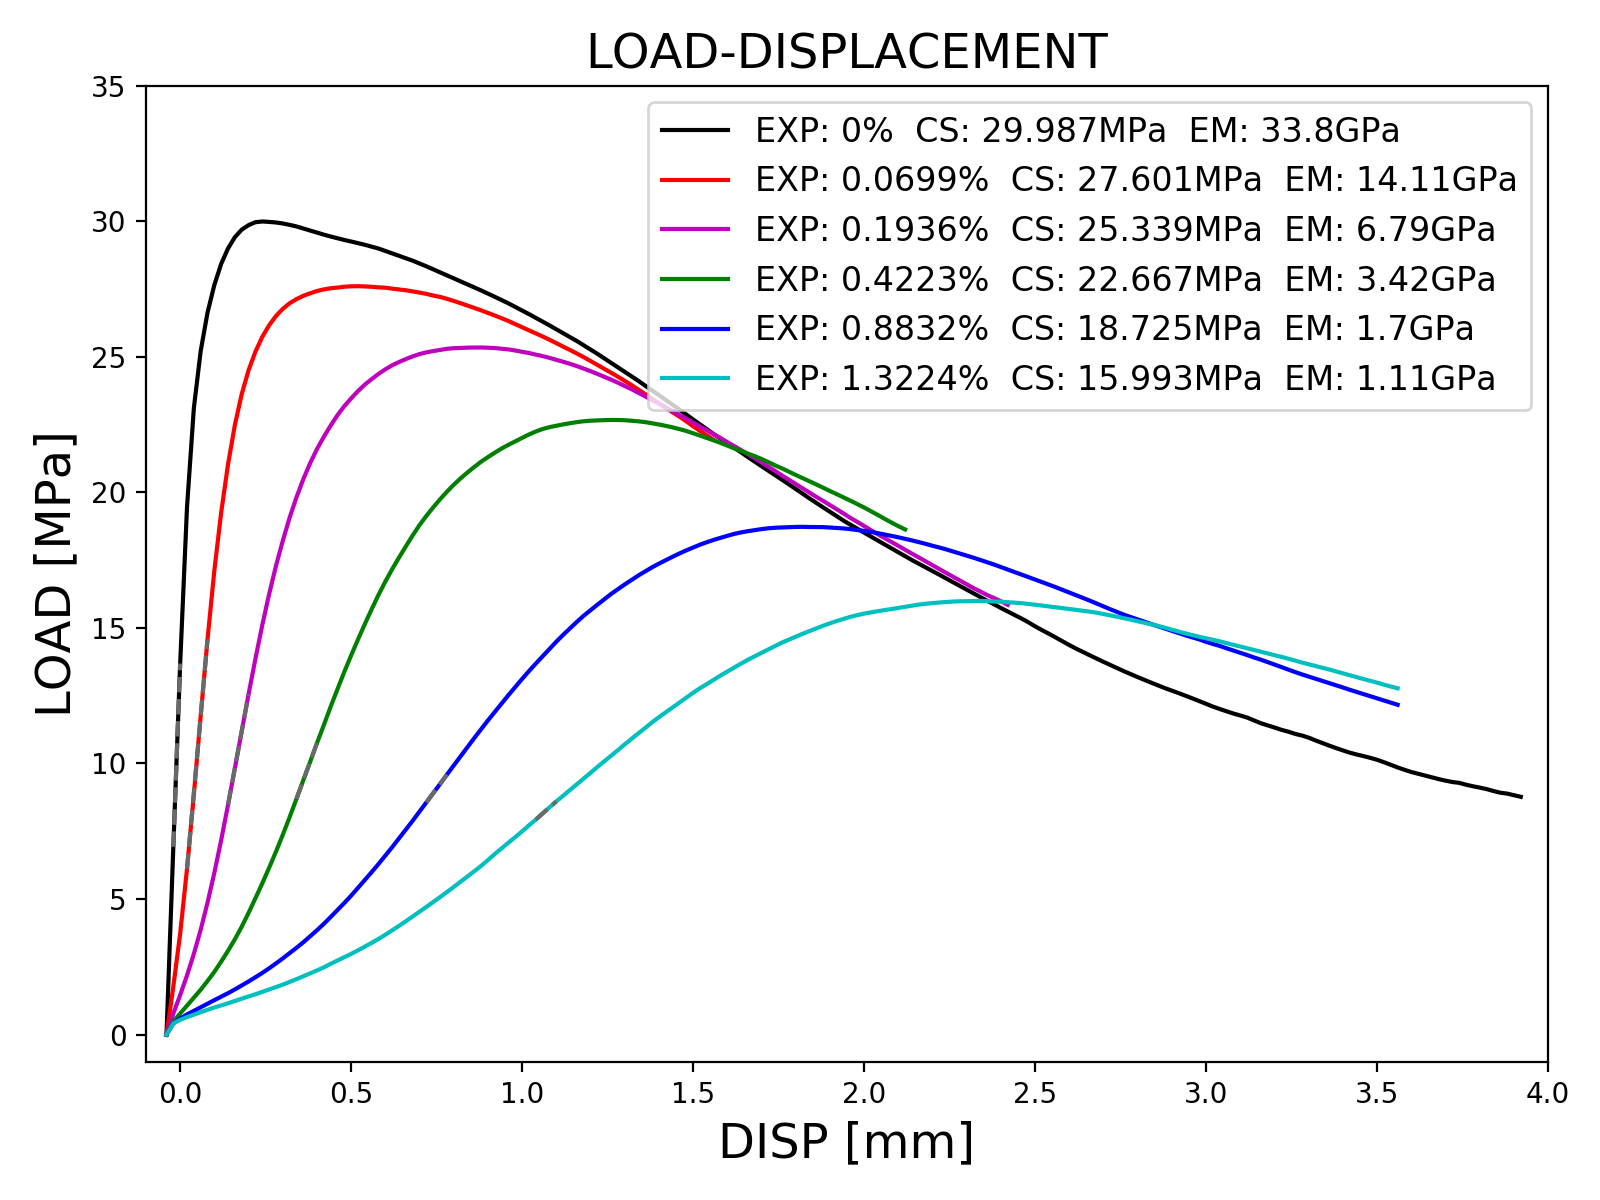
\includegraphics[width=0.8\linewidth]{Files/exp_3D/ASR/S13A30P75FIX-LOAD-DISPLACEMENT.png}
    \caption{LOAD-DISPLACEMENT(Fix Boundary Condition)}
    \label{fig:S13A30P75FIX-LOAD-DISPLACEMENT}
\end{figure}

\begin{figure}[ht!]
    \centering
    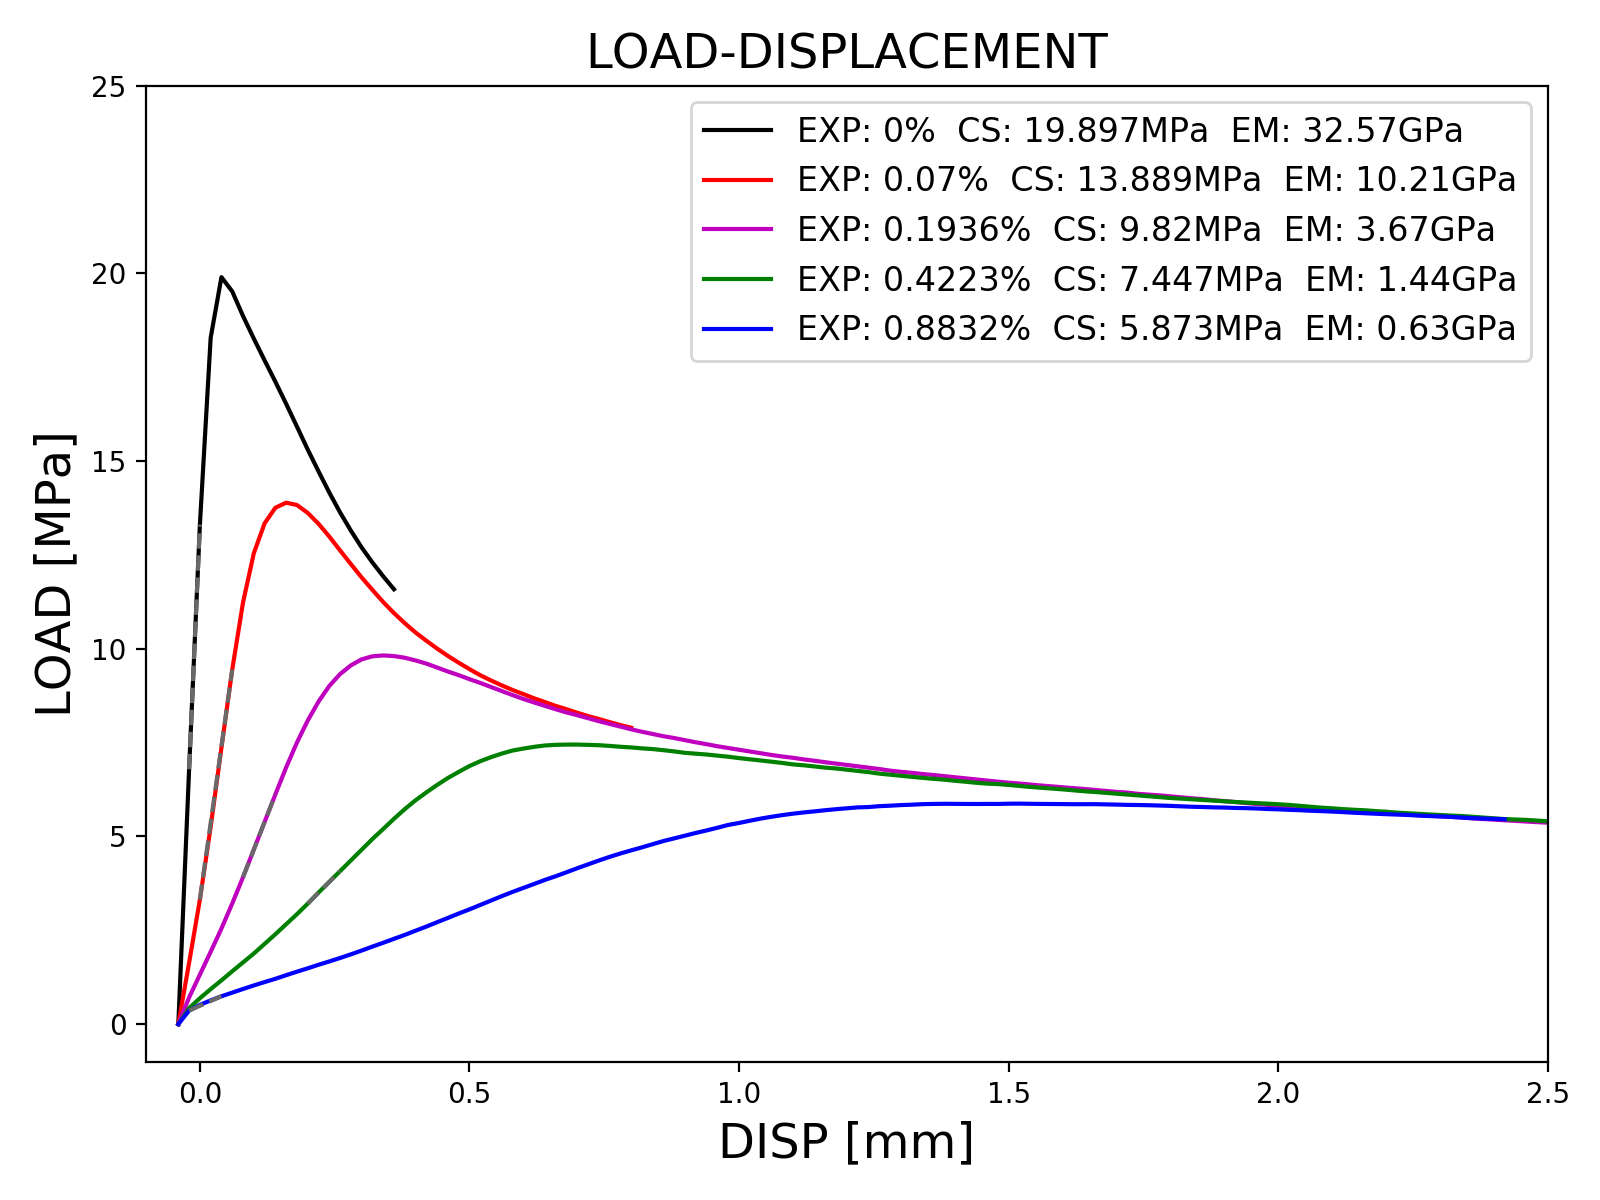
\includegraphics[width=0.8\linewidth]{Files/exp_3D/ASR/S13A30P75FREE-LOAD-DISPLACEMENT.png}
    \caption{LOAD-DISPLACEMENT(Free Boundary Condition)}
    \label{fig:S13A30P75FREE-LOAD-DISPLACEMENT}
\end{figure}

%% ASR_A30_P75 Surface Crack

\begin{figure}[ht!]
    \centering
    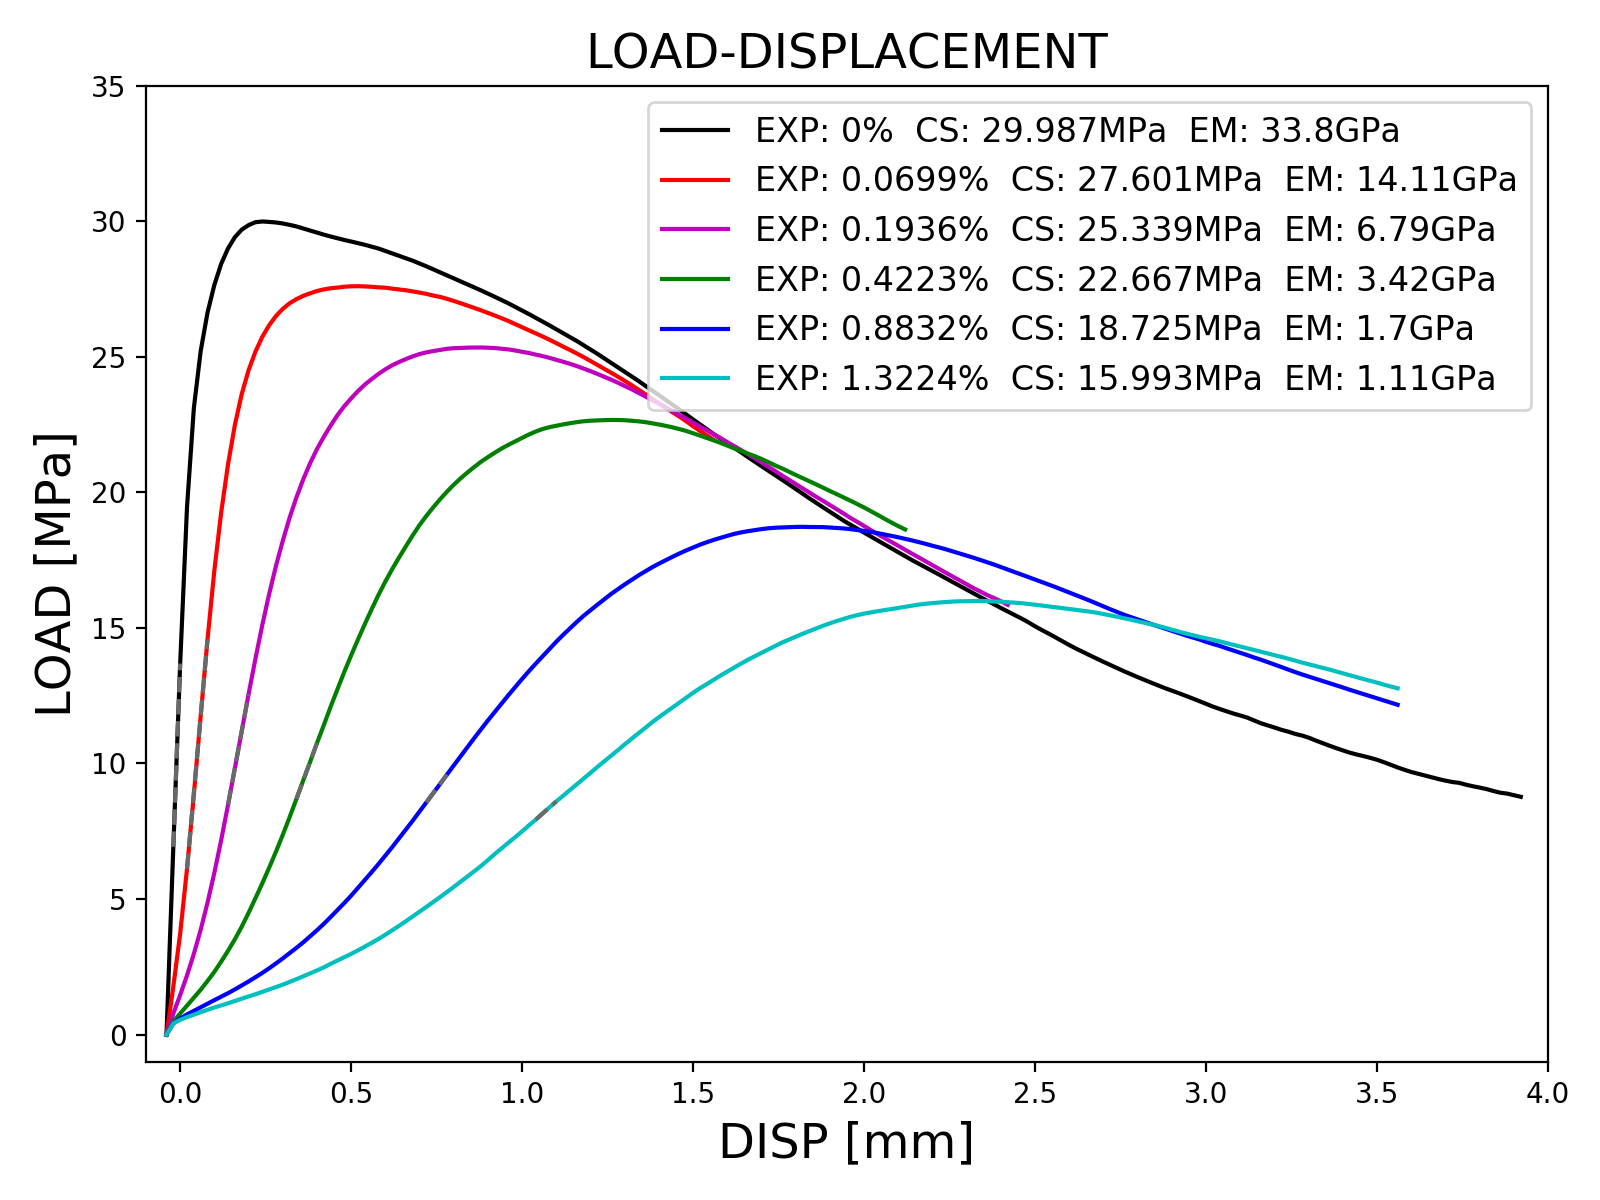
\includegraphics[width=0.8\linewidth]{Files/exp_3D/ASR/S13A30P75FIX-LOAD-DISPLACEMENT.png}
    \caption{LOAD-DISPLACEMENT(Fix Boundary Condition)}
    \label{fig:S13A30P75FIX-LOAD-DISPLACEMENT}
\end{figure}

\begin{figure}[ht!]
\centering
    %*******
    %*******
    \begin{subfigure}{.5\textwidth}
      \centering
      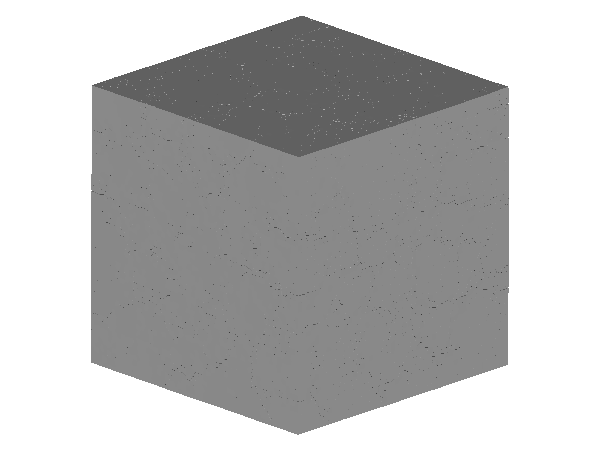
\includegraphics[width=0.5\linewidth]{Files/exp_3D/ASR/A30P75_1_3d.png}
      \caption{0.0699\% Expansion\\3D Surface Crack}
    \end{subfigure}%
    %*******
    \begin{subfigure}{.5\textwidth}
      \centering
      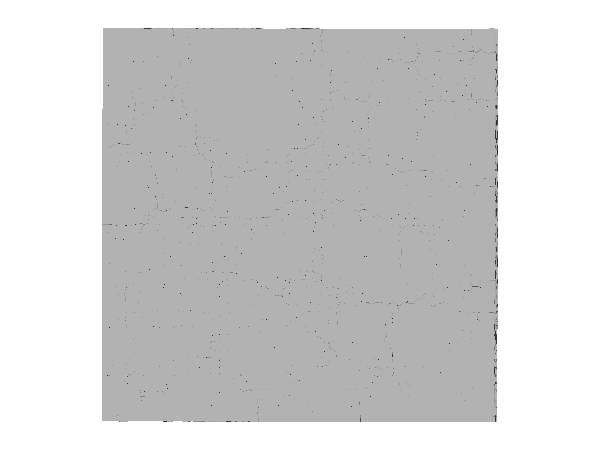
\includegraphics[width=0.5\linewidth]{Files/exp_3D/ASR/A30P75_1_3ds.png}
      \caption{0.0699\% Expansion\\3D Surface Crack (One Side)}
    \end{subfigure}%
    %*******

    %*******
    \begin{subfigure}{.5\textwidth}
      \centering
      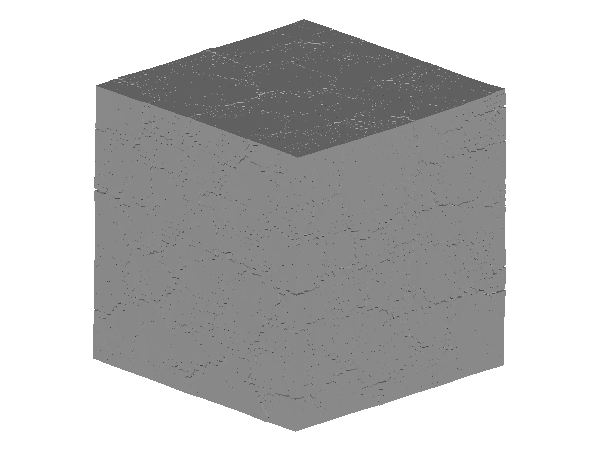
\includegraphics[width=0.5\linewidth]{Files/exp_3D/ASR/A30P75_2_3d.png}
      \caption{0.1936\% Expansion\\3D Surface Crack}
    \end{subfigure}%
    %*******
    \begin{subfigure}{.5\textwidth}
      \centering
      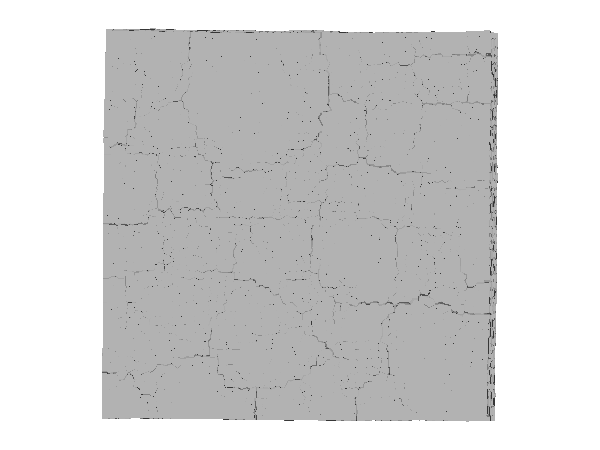
\includegraphics[width=0.5\linewidth]{Files/exp_3D/ASR/A30P75_2_3ds.png}
      \caption{0.1936\% Expansion\\3D Surface Crack (One Side)}
    \end{subfigure}%
    %*******

    %*******
    \begin{subfigure}{.5\textwidth}
      \centering
      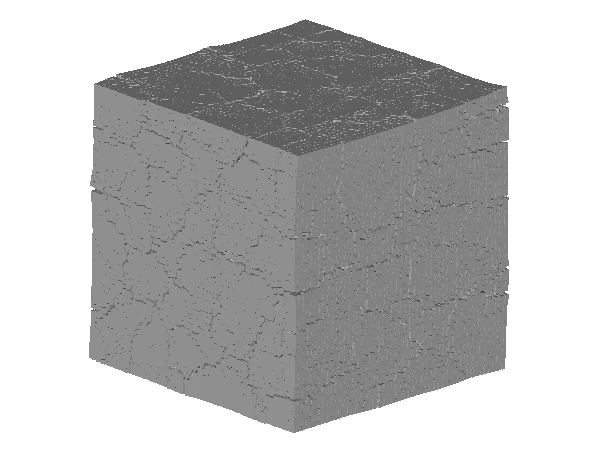
\includegraphics[width=0.5\linewidth]{Files/exp_3D/ASR/A30P75_3_3d.png}
      \caption{0.4223\% Expansion\\3D Surface Crack}
    \end{subfigure}%
    %*******
    \begin{subfigure}{.5\textwidth}
      \centering
      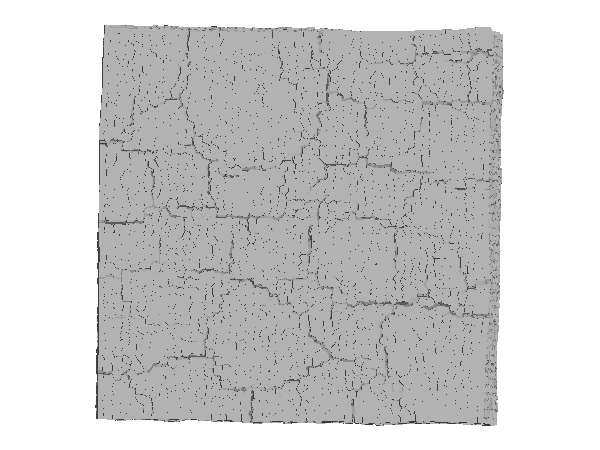
\includegraphics[width=0.5\linewidth]{Files/exp_3D/ASR/A30P75_3_3ds.png}
      \caption{0.4223\% Expansion\\3D Surface Crack (One Side)}
    \end{subfigure}%
    %*******

    %*******
    \begin{subfigure}{.5\textwidth}
      \centering
      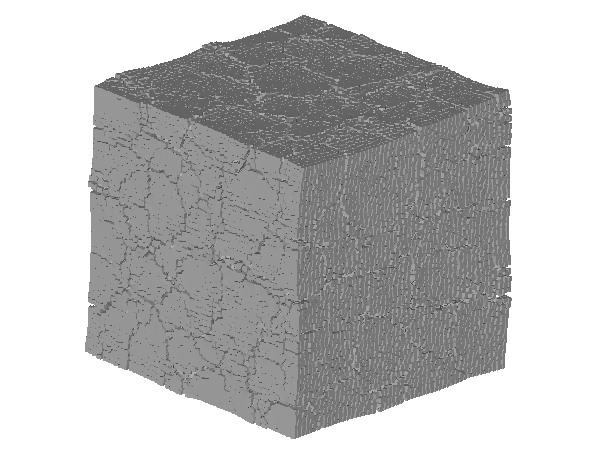
\includegraphics[width=0.5\linewidth]{Files/exp_3D/ASR/A30P75_4_3d.png}
      \caption{0.8832\% Expansion\\3D Surface Crack}
    \end{subfigure}%
    %*******
    \begin{subfigure}{.5\textwidth}
      \centering
      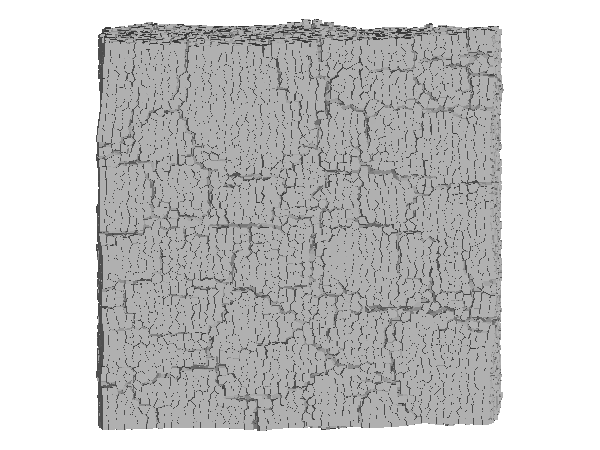
\includegraphics[width=0.5\linewidth]{Files/exp_3D/ASR/A30P75_4_3ds.png}
      \caption{0.8832\% Expansion\\3D Surface Crack (One Side)}
    \end{subfigure}%
    %*******

    %*******
    \begin{subfigure}{.5\textwidth}
      \centering
      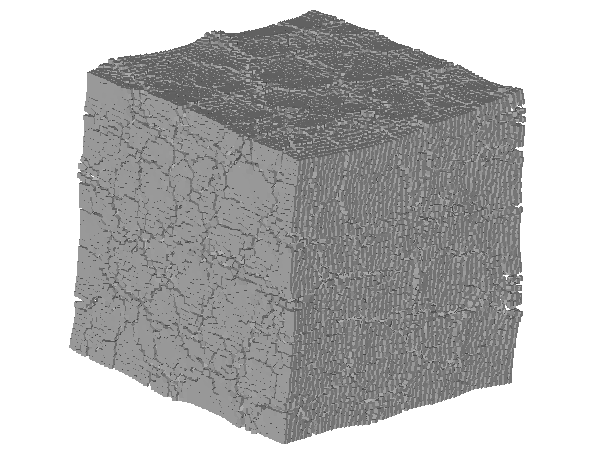
\includegraphics[width=0.5\linewidth]{Files/exp_3D/ASR/A30P75_5_3d.png}
      \caption{1.3224\% Expansion\\3D Surface Crack}
    \end{subfigure}%
    %*******
    \begin{subfigure}{.5\textwidth}
      \centering
      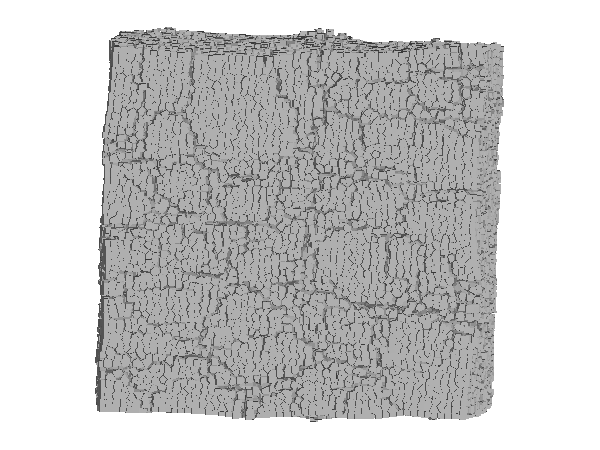
\includegraphics[width=0.5\linewidth]{Files/exp_3D/ASR/A30P75_5_3ds.png}
      \caption{1.3224\% Expansion\\3D Surface Crack (One Side)}
    \end{subfigure}%
    %*******

\caption{3D Surface Cracking Pattern}
\label{fig:A30_3Dcrack}
\end{figure}

\begin{figure}[ht!]
\centering
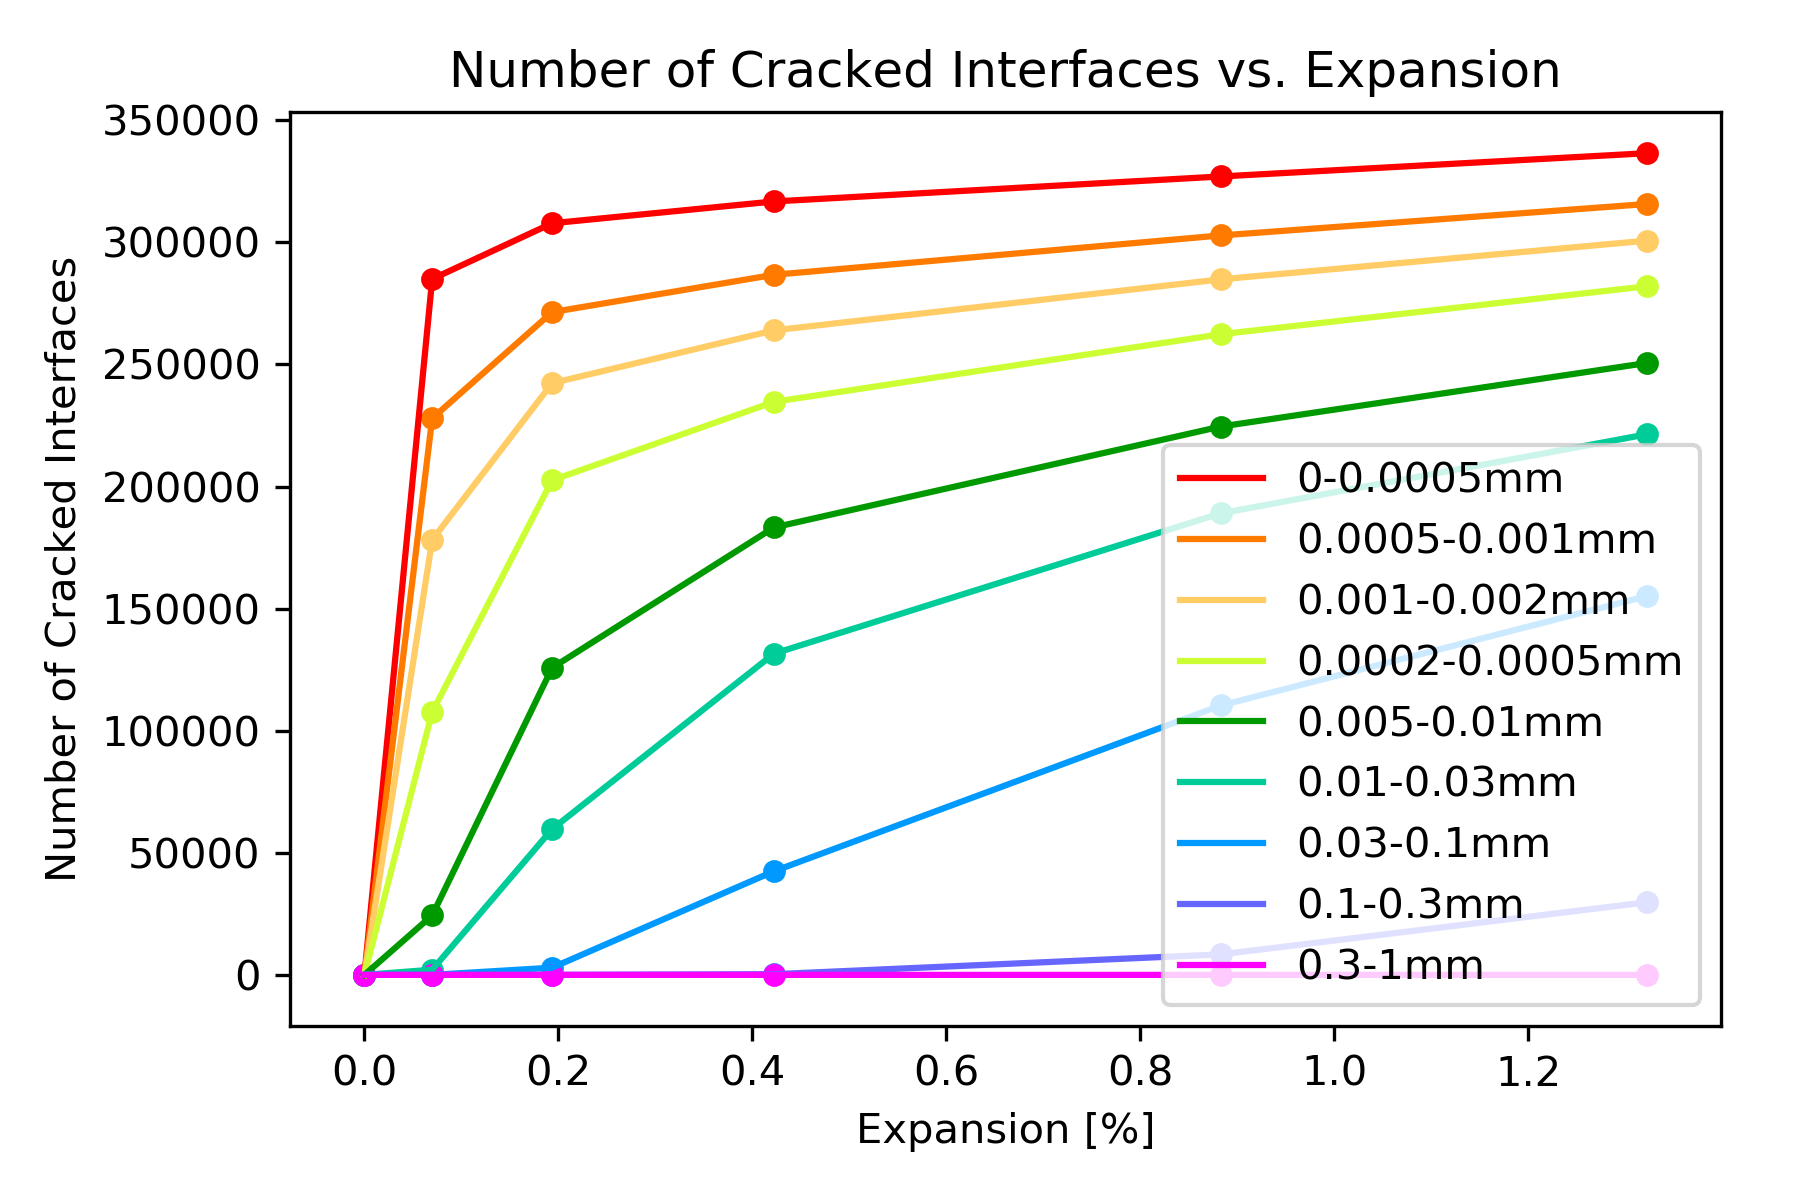
\includegraphics[width=.8\linewidth]{Files/interface/A30P75CRACK.png}
  \caption{Number of Cracked Interface vs. Expansion}
  \label{A30P75CRACK}
\end{figure}
